<<<<<<< HEAD
\documentclass[english, a4paper,11pt]{article}
\usepackage[latin1]{inputenc}
\usepackage[T1]{fontenc}
\usepackage{bbm}
\usepackage{amsmath}
\usepackage{indentfirst}
\usepackage{fullpage}
\usepackage{url}
\usepackage{graphicx}
\usepackage{geometry}
\geometry{verbose,tmargin=3cm,bmargin=2cm,lmargin=2cm,rmargin=2cm}
\usepackage{babel}
\usepackage[center,footnotesize]{caption}
\usepackage[section]{placeins}
\usepackage{subfig}
\title{Solutions - Series 4}
\date{October 11, 2011}
\author{Genomics and bioinformatics - Week 4}
\begin{document}
\maketitle





\section{Sequence alignment}
\emph{Match:}  \texttt{+1}, \emph{Mismatch:} \texttt{-1}, \emph{Gap:} \texttt{-2}
Sequence 1: \texttt{GAATTCAGA}
Sequence 2: \texttt{GGATCGA}.\\

\subsection{Initialization}
Create a matrix with \texttt{m + 1} columns and \texttt{n + 1} rows where \texttt{m} and \texttt{n} correspond to the sizes of Sequences 1 and 2, respectively. \\

\subsection{Scoring}
Using the given scoring scheme, at each cell, 3 scores are calculated:
\begin{itemize}
\item Upper neighbor score + Gap cost
\item Left neighbor score + Gap cost
\item Upper-left neighbor score + Match score (if nucleotides match), \emph{OR} 
Upper-left neighbor score + Mismatch cost (if nucleotides do not match)
\end{itemize}
The highest score is retained and the arrow is labelled. Here is the resulting scoring matrix: \\
\begin{center}
\includegraphics[width=0.6\textwidth]{scoring.png}\\
\end{center}

\subsection{Backtracking}
The process of deduction of the best alignment from the score matrix is known as traceback. 
The traceback begins with the last cell to be filled, i.e. the bottom-right cell, and is 
completed when the first, i.e. the top-left cell of the matrix is reached. Several 
traceback paths are possible. The solution resulting in the best final score is selected 
to deduce the optimum alignment. It is possible to have more than one optimum alignment. 
A traceback path for the scoring matrix generated in Step 2 is highlighted below.

\begin{center}
\includegraphics[width=0.6\textwidth]{backtracking.png}
\end{center}

\subsection{Alignment}

After backtracking, the optimal alignment is easy to recover using the following rule:

 \emph{Left} = Deletion , \emph{Up} = Insertion, and \emph{Diagonal} = Match 

The optimum alignment for the two sequences \texttt{GAATTCAGA} and \texttt{GGATCGA} is,

\begin{center}
\includegraphics[width=0.2\textwidth]{alignment.png}
\end{center}










\section{Pair HMM}

\subsection{Finding the Emission and Transtion Probabilities}
The corresponding HMM is given by the following figure .


\begin{centering}
\includegraphics[width=0.3\textwidth]{HMM.jpg}

\end{centering}





If we consider all probability values with respect to a random model
in log-odds
$$S(x,y)=log\frac{p(x,y)}{p(x)\; p(y)}$$ where $p(x)$ is the probability of choosing one nucleotide at random. So, $p(x)=1/4$.

$S(x,y)=1$ for match and $s(x,y)=-1$ for mismatch

$p(x,y)=p(x|y)\;p(y)$ where $p(x|y)$ is the prbability of $x$ conditioned on $y$. Therefore,

$$S(x,y)=log\frac{p(x|y)}{p(x)}$$ 
So, we can find the  emision probability values with this following equation

$$p(x|y)=2^{S(x,y)}\;p(x)$$


The emission prbabiliy matrix is given by


\begin{table}[ht]
\caption{Emission Probability Matrix} % title of Table
\centering % used for centering table
\begin{tabular}{c c c c c} % centered columns (4 columns)

-- & A  & C & G & T \\ [0.5ex] % inserts table
%heading

A & 1/2 & 1/8 & 1/8 & 1/8 \\ % inserting body of the table
C & 1/8  & 1/2 & 1/8 & 1/8 \\
G & 1/8 & 1/8 & 1/2 & 1/8 \\
T & 1/8 & 1/8 & 1/8 & 1/2 \\ [1ex] % [1ex] adds vertical space

\hline %inserts single line
\end{tabular}
\label{table:nonlin} % is used to refer this table in the text
\end{table}

and  $q(x,_)=q(_,y)=1/4$
and the Transition Prbabilities are

$\delta=1/4$ and $\epsilon=\delta$.

\subsection{Constructing the Three Matrices (VM,VD and VI)}

Then we can construct the three matrices for VM, VD and VI by the Viterbi
algorithm.

Matrix $V_M$:
%\begin{figure}[h]
\begin{center}
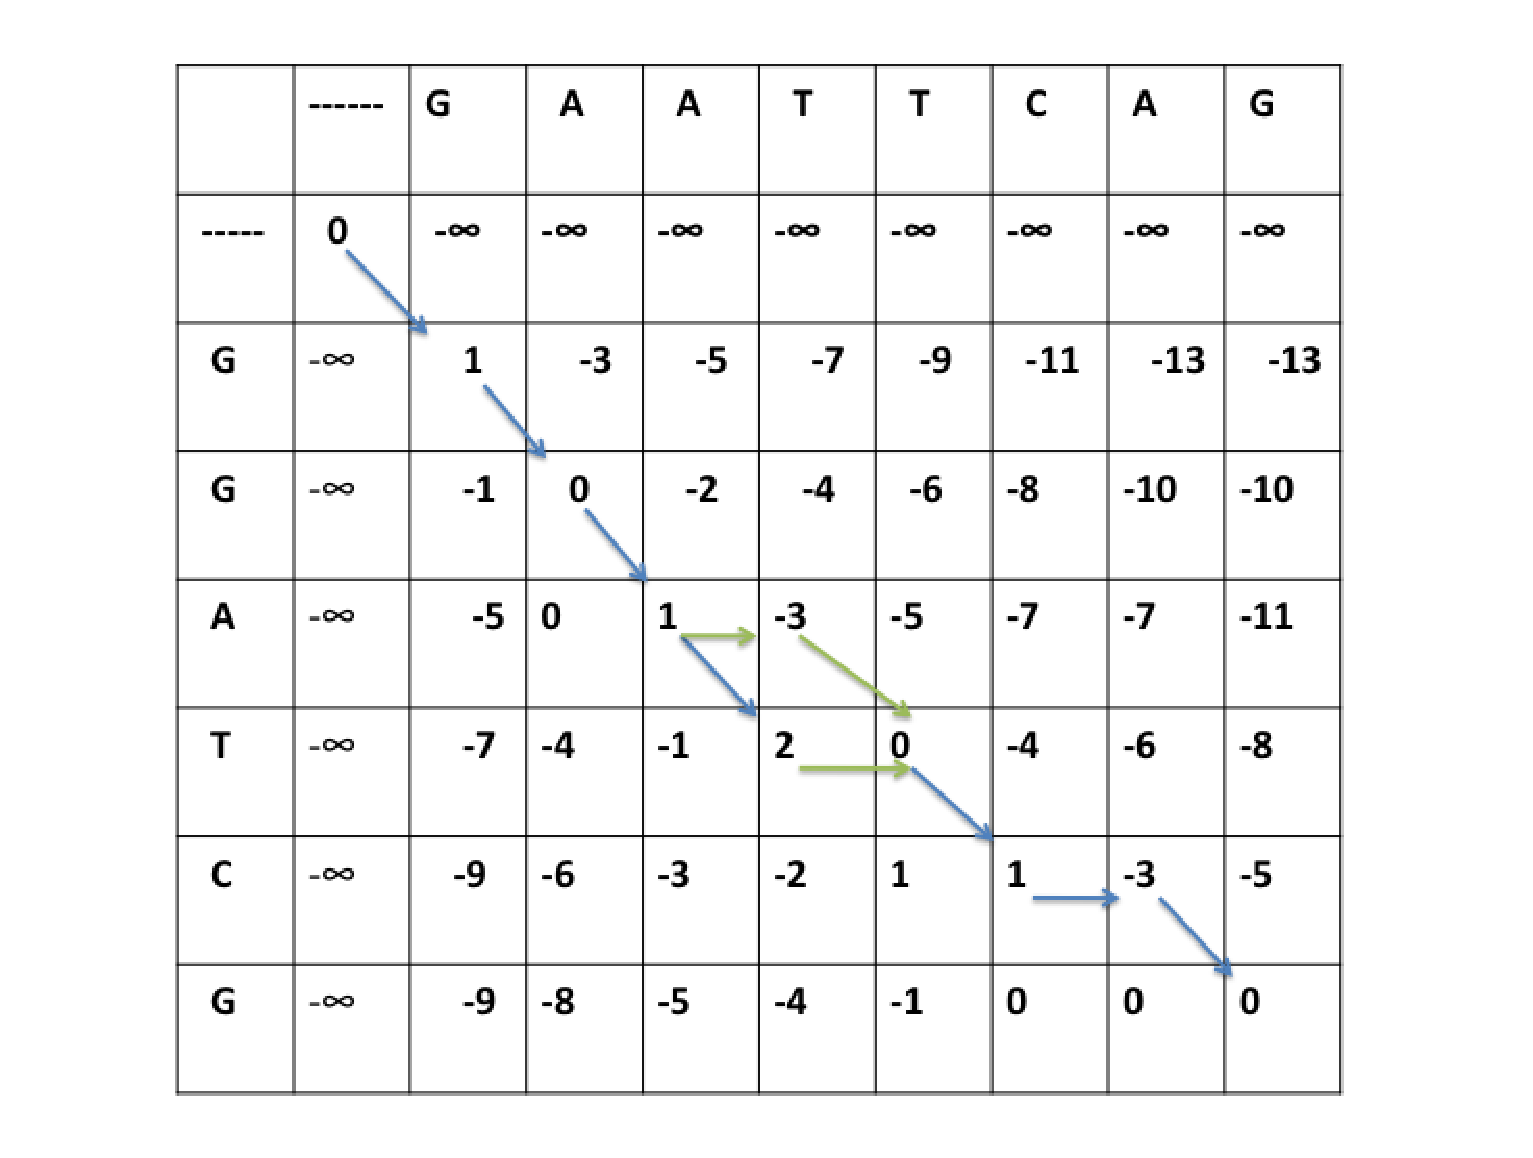
\includegraphics[width=0.8\textwidth]{Slide1}
%\caption{The matrix for the match state VM}
\end{center}
%\end{figure}

\newpage
Matrix $V_D$:
%\begin{figure}[h]
\begin{center}
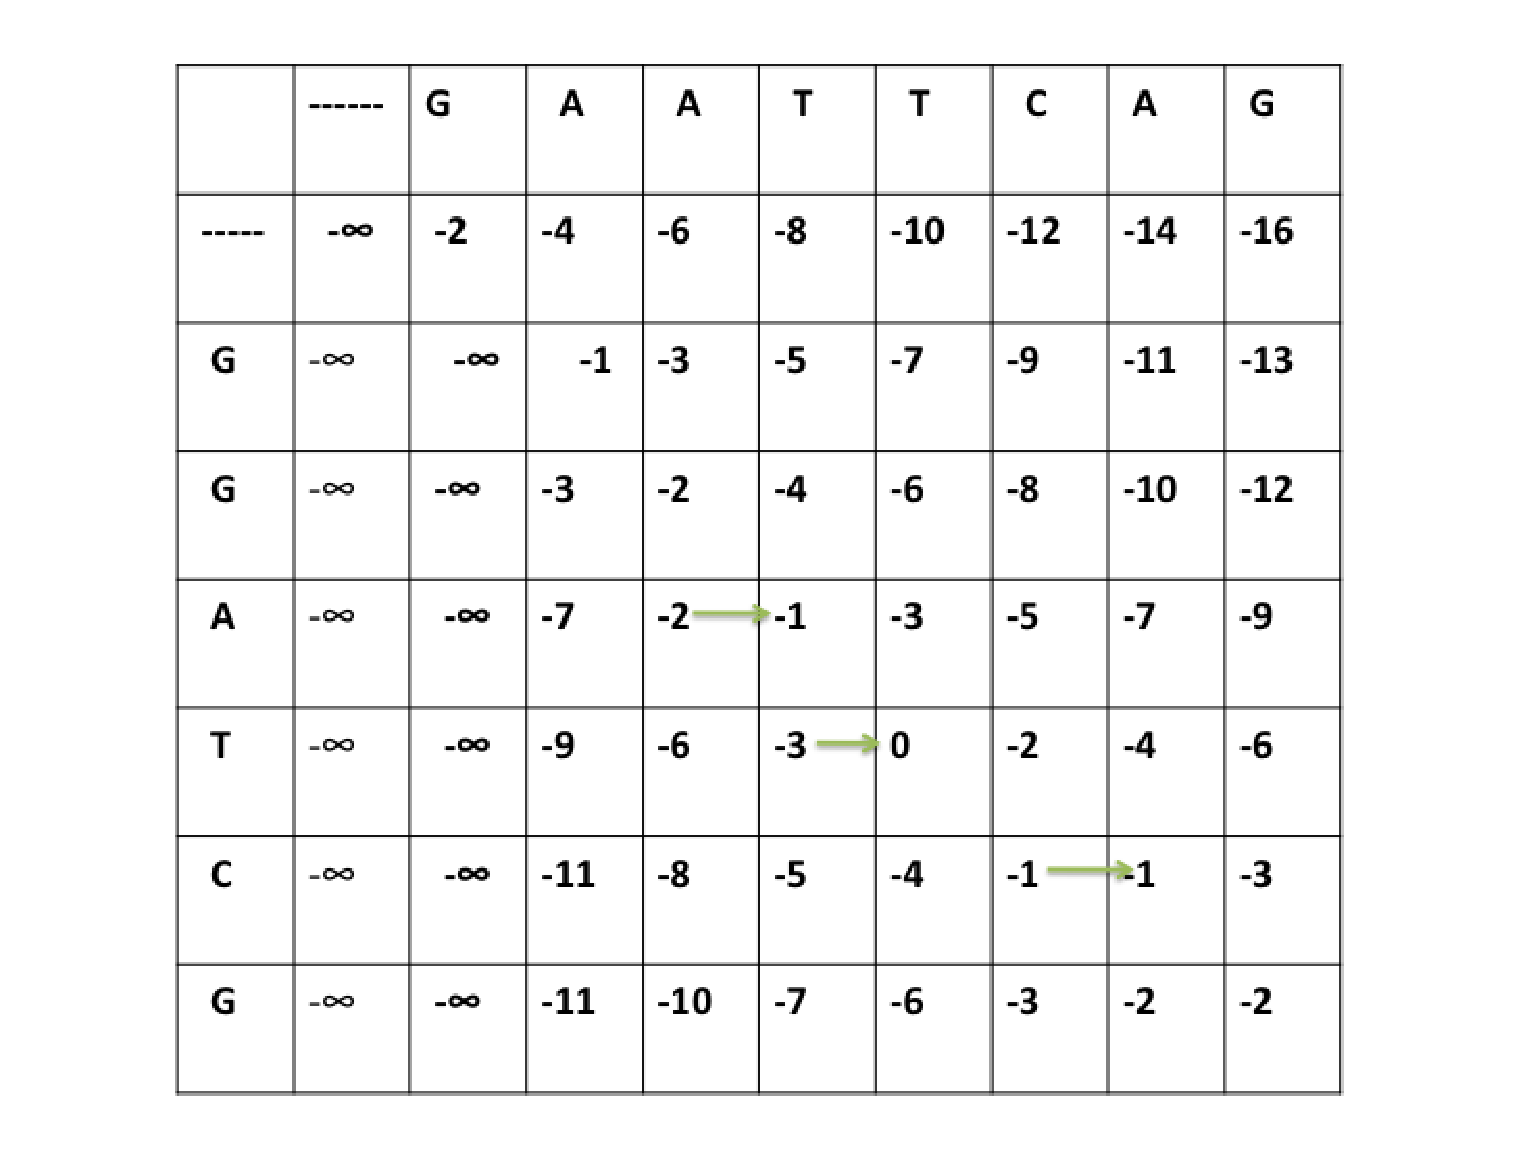
\includegraphics[width=0.8\textwidth]{Slide2}
%\caption{Matrix for deletion state VD}
\end{center}
%\end{figure}

Matrix $V_I$:
%\begin{figure}[h]
\begin{center}

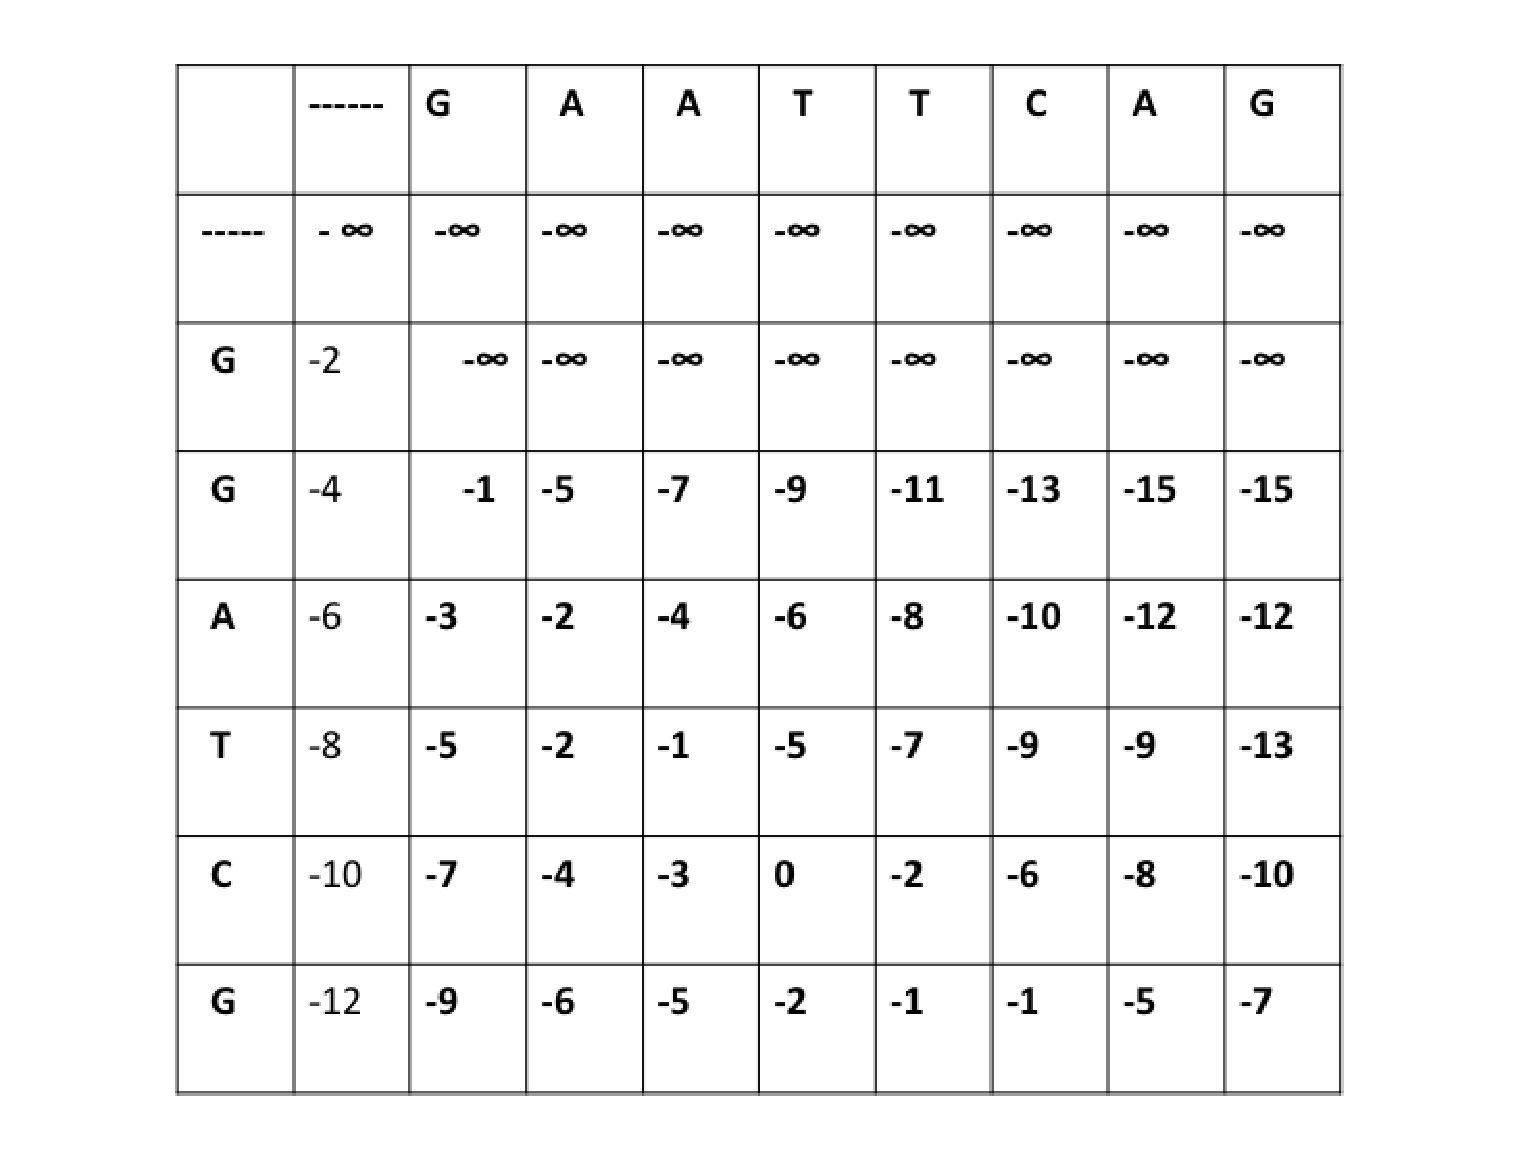
\includegraphics[width=0.8\textwidth]{Slide3}
%\caption{Matrix for insertion state VI}
\end{center}
%\end{figure}

\subsection{Deducing the Alignments}

The final matrix is formed by taking maximum value from the three elements of each matrix.
\newpage
Alignment by backtracking:
%\begin{figure}[ht]
\begin{center}
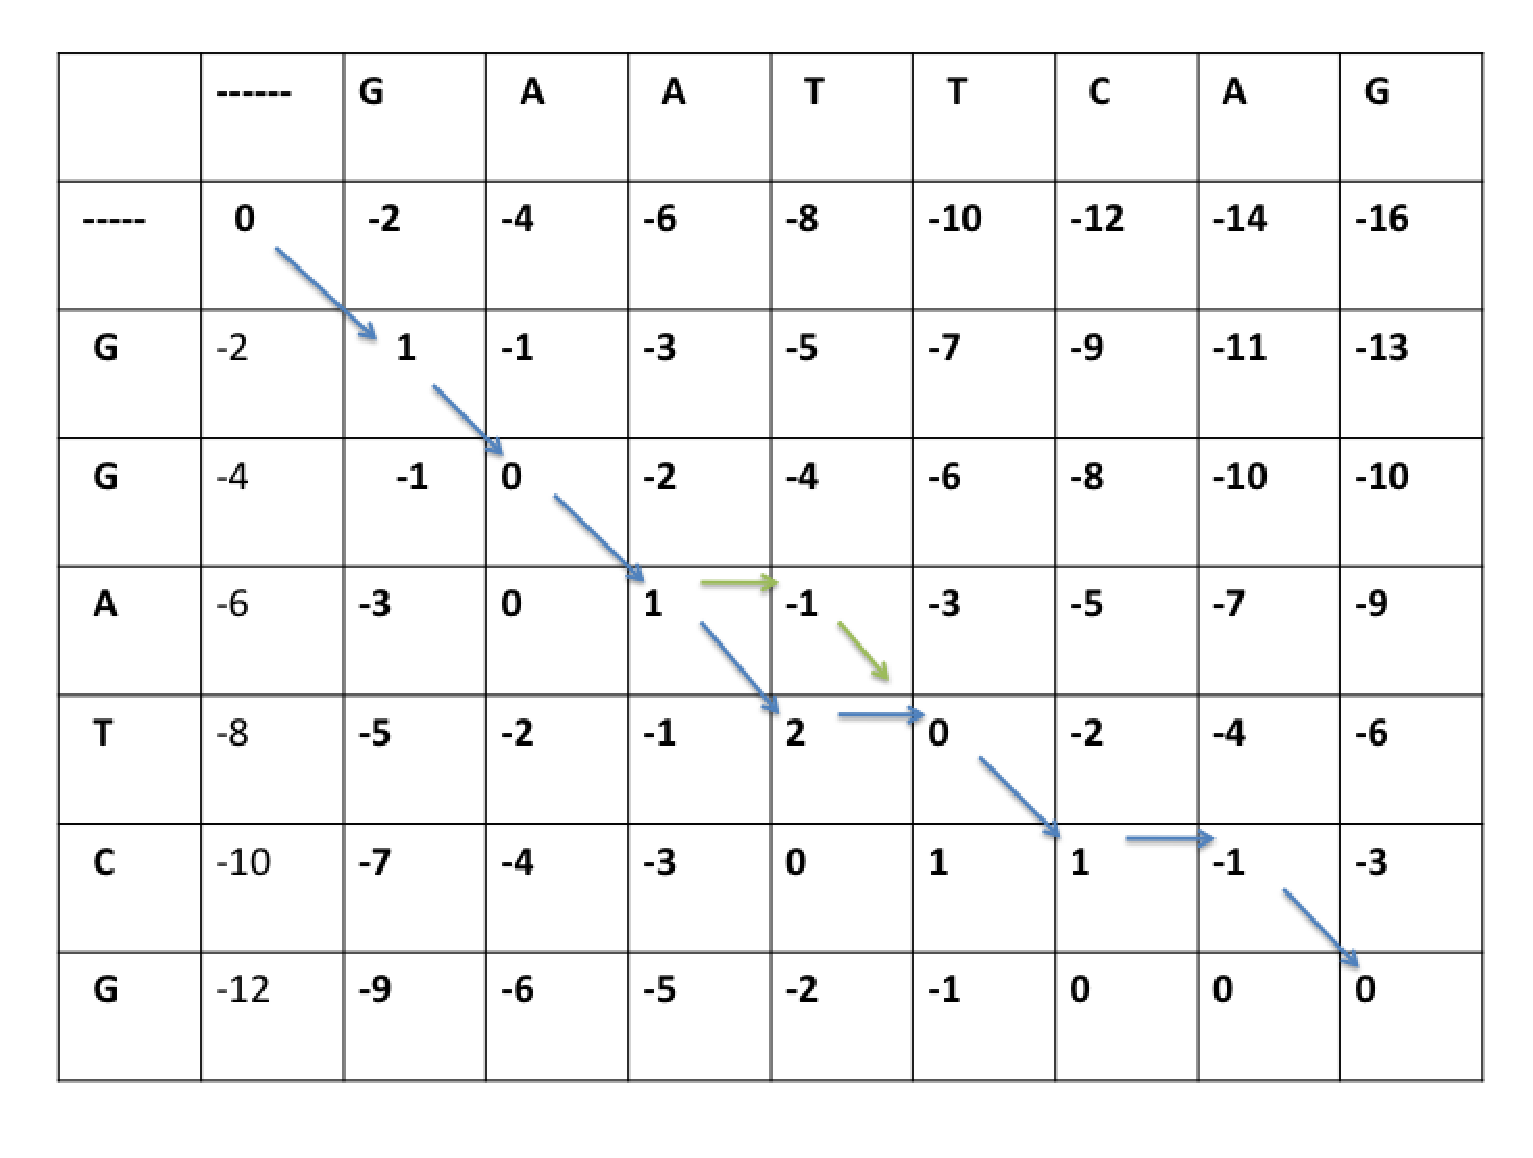
\includegraphics[width=0.8\textwidth]{Slide4}
%\caption{Alignment by backtracking}
\end{center}
%\end{figure}

There are two possible optimal alignments.

%\begin{figure}[h]
\begin{center}
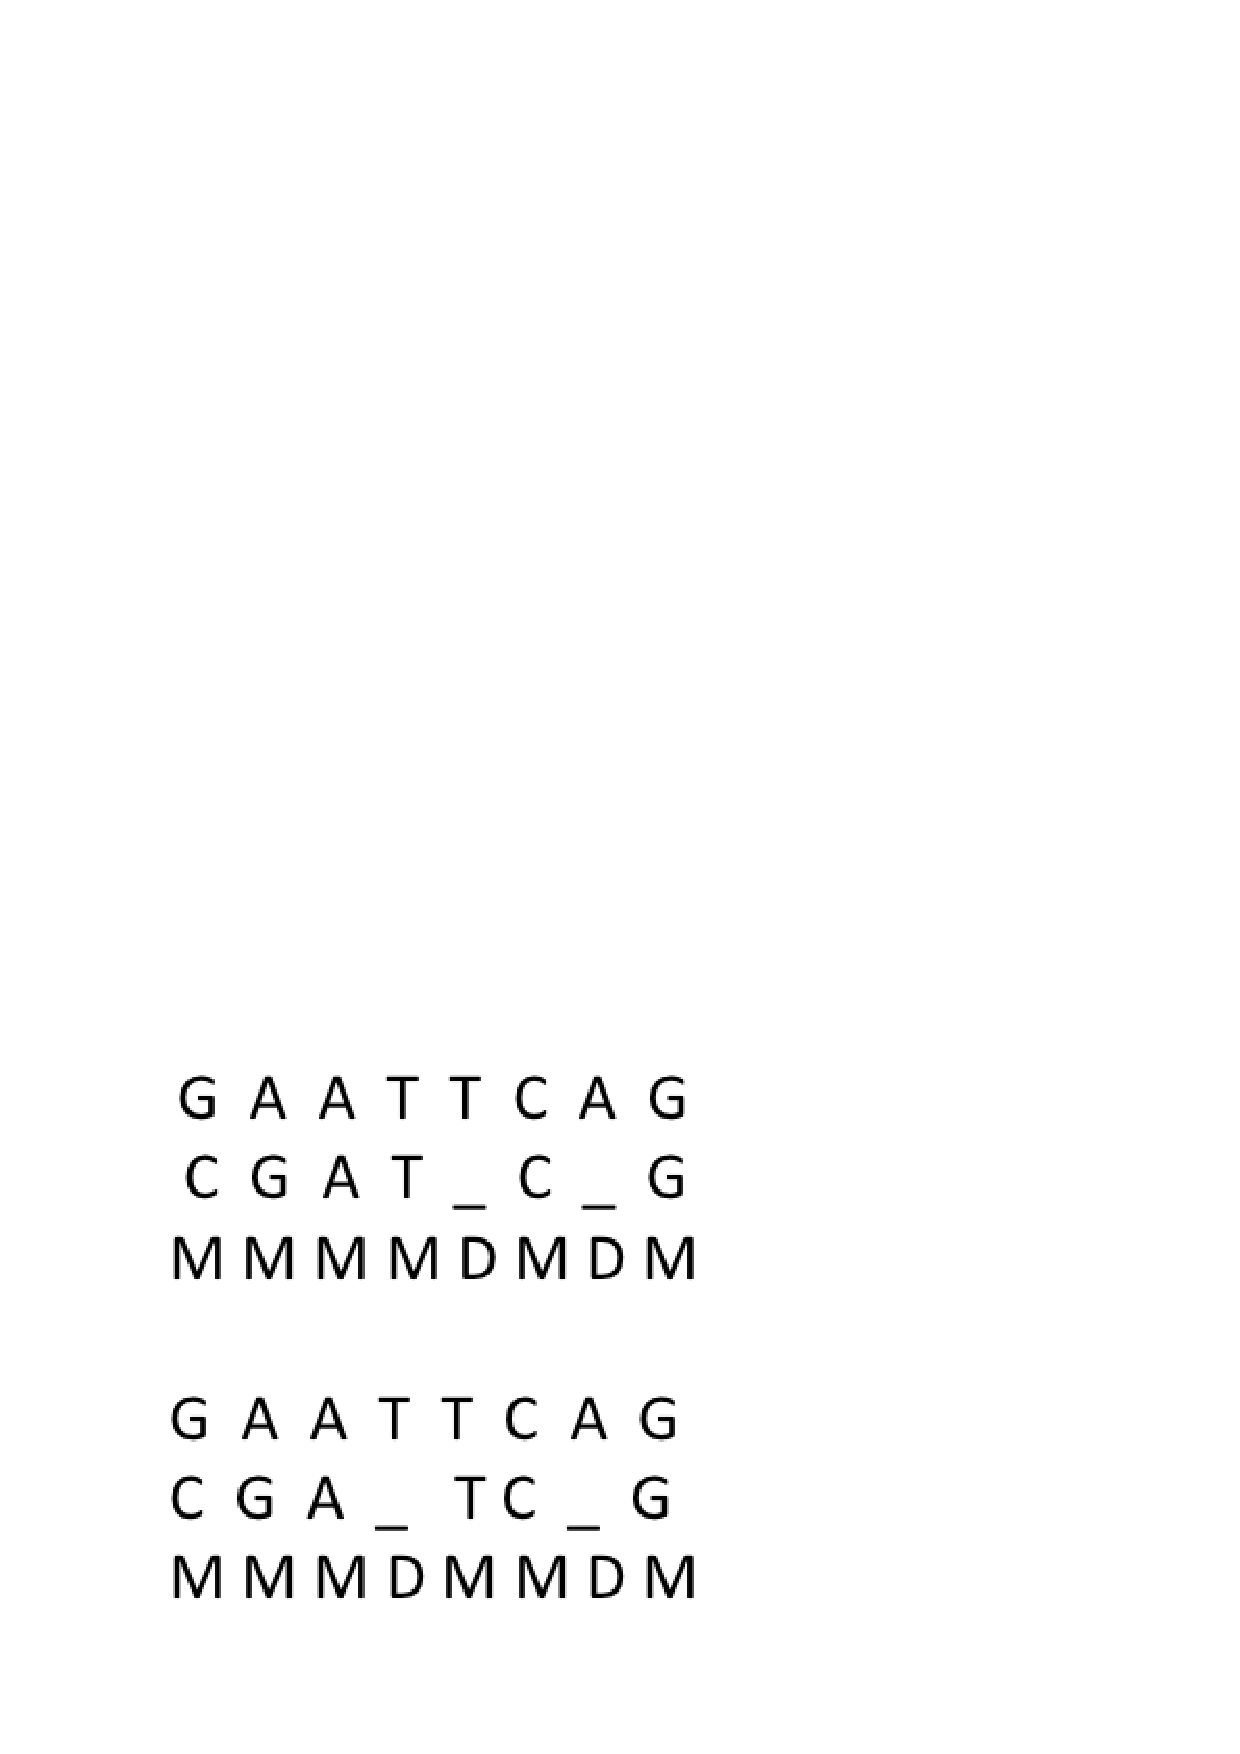
\includegraphics[width=0.8\textwidth]{alignment2.png}
\end{center}
%\caption{The alignments}
%\end{figure}

\end{document}
=======
\documentclass[english, a4paper,11pt]{article}
\usepackage[latin1]{inputenc}
\usepackage[T1]{fontenc}
\usepackage{bbm}
\usepackage{amsmath}
\usepackage{indentfirst}
\usepackage{fullpage}
\usepackage{url}
\usepackage{graphicx}
\usepackage{geometry}
\geometry{verbose,tmargin=3cm,bmargin=2cm,lmargin=2cm,rmargin=2cm}
\usepackage{babel}
\usepackage[center,footnotesize]{caption}
\usepackage[section]{placeins}
\usepackage{subfig}
\title{Solutions - Series 4}
\date{October 11, 2011}
\author{Genomics and bioinformatics - Week 4}
\begin{document}
\maketitle




\section{Sequence alignment}
\emph{Match:}  \texttt{+1}, \emph{Mismatch:} \texttt{-1}, \emph{Gap:} \texttt{-2}
Sequence 1: \texttt{GAATTCAG}
Sequence 2: \texttt{GGATCG}.\\

\subsection{Initialization}
Create a matrix with \texttt{m + 1} columns and \texttt{n + 1} rows where \texttt{m} and \texttt{n} correspond to the sizes of Sequences 1 and 2, respectively. \\

\subsection{Scoring}
Using the given scoring scheme, at each cell, 3 scores are calculated:
\begin{itemize}
\item Upper neighbor score + Gap cost
\item Left neighbor score + Gap cost
\item Upper-left neighbor score + Match score (if nucleotides match), \emph{OR} 
Upper-left neighbor score + Mismatch cost (if nucleotides do not match)
\end{itemize}
The highest score is retained and the arrow is labelled. Here is the resulting scoring matrix: \\
\begin{center}
\includegraphics[width=0.6\textwidth]{scoring.png}\\
\end{center}

\subsection{Backtracking}
The process of deduction of the best alignment from the score matrix is known as traceback. 
The traceback begins with the last cell to be filled, i.e. the bottom-right cell, and is 
completed when the first, i.e. the top-left cell of the matrix is reached. Several 
traceback paths are possible. The solution resulting in the best final score is selected 
to deduce the optimum alignment. It is possible to have more than one optimum alignment. 
A traceback path for the scoring matrix generated in Step 2 is highlighted below.

\begin{center}
\includegraphics[width=0.6\textwidth]{backtracking.png}
\end{center}

\subsection{Alignment}

After backtracking, the optimal alignment is easy to recover using the following rule:

 \emph{Left} = Deletion , \emph{Up} = Insertion, and \emph{Diagonal} = Match 

The optimum alignment for the two sequences \texttt{GAATTCAG} and \texttt{GGATCG} is,

\begin{center}
\includegraphics[width=0.2\textwidth]{alignment.png}
\end{center}











\section{Pair HMM}

The corresponding HMM is given by figure \ref{fig:hmmmodel}.

\begin{figure}
\begin{centering}
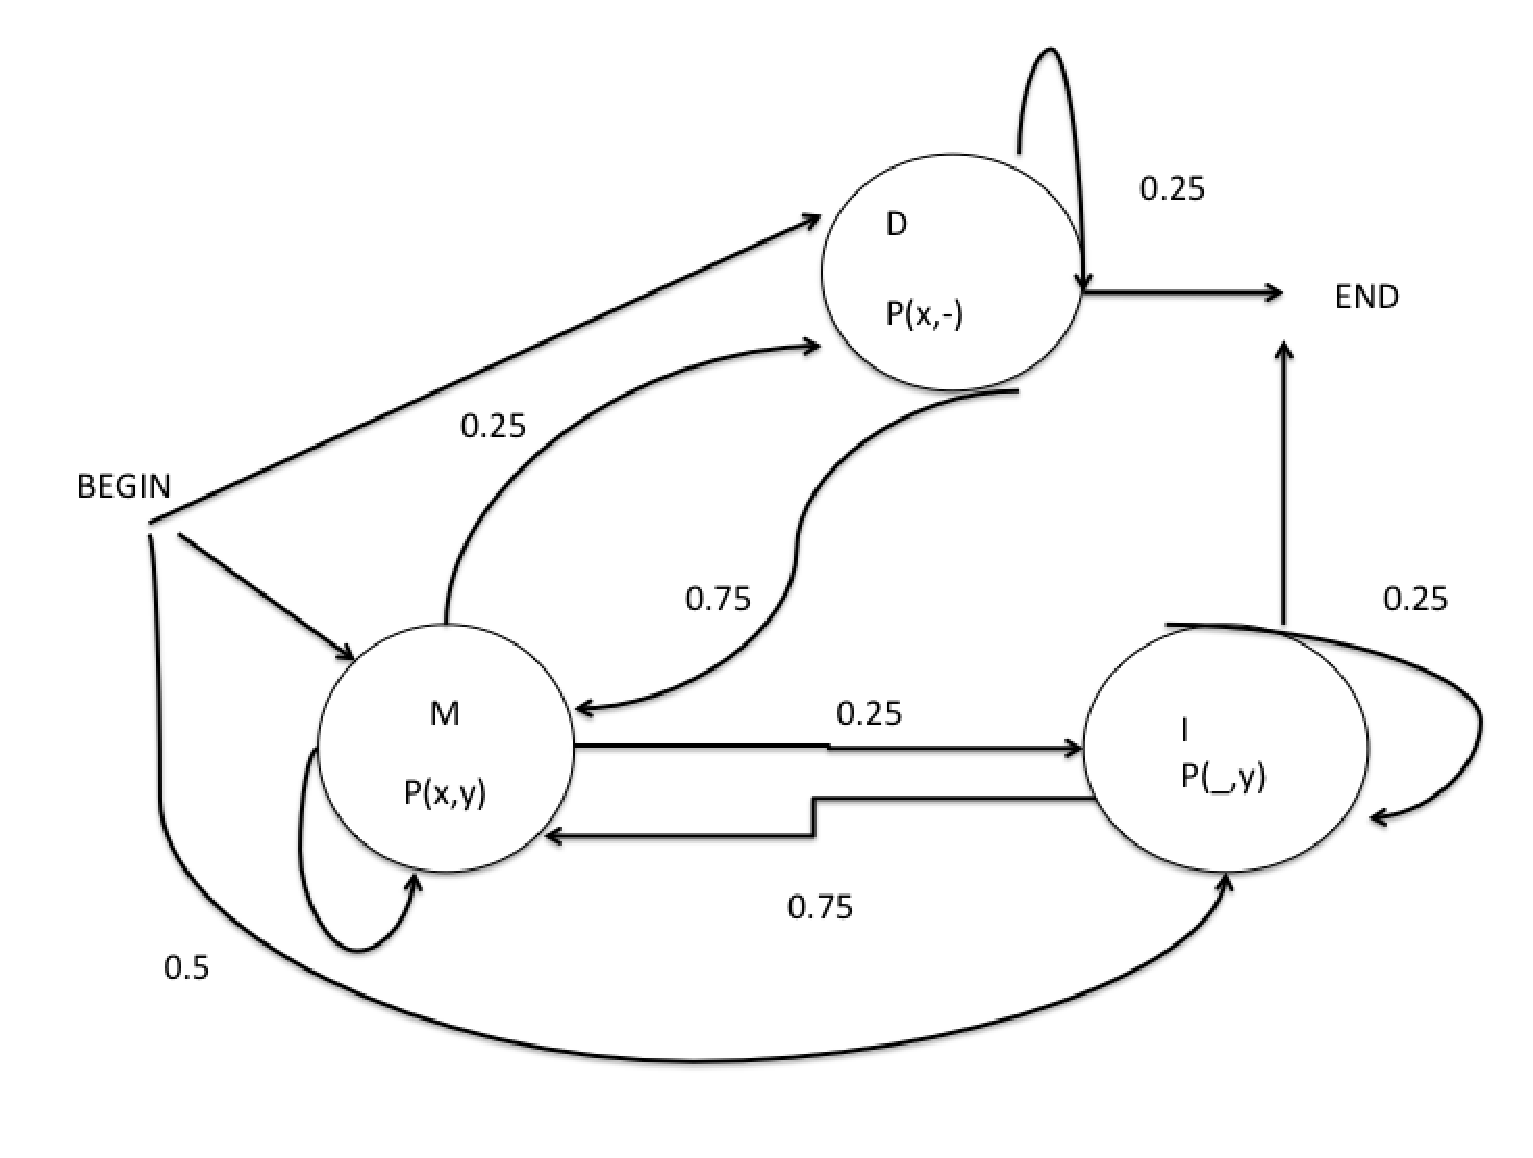
\includegraphics[width=4in]{Slide5}
\par\end{centering}
\caption{The HMM model for sequence alignment}
\label{fig:hmmmodel}
\end{figure}

where $p(x,y)=0.125$ and $p(x,y)=0.04$ for mismatch

$p(x,\_)=q(\_,y)=0.25$

If we consider all probability values with respect to a random model
in log-odds
$$S(x,y)=log\frac{p(x,y)}{p(x)\; p(y)}$$

$S(x,y)=1$ for match and $s(x,y)=-1$ for mismatch

\begin{figure}
\begin{centering}
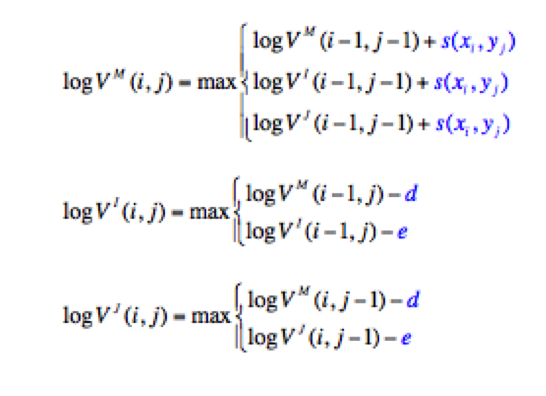
\includegraphics[width=3in]{Viterbi}
\par\end{centering}
\caption{Viterbi Algorithm}
\end{figure}

The we can construct the three matrices for VM, VX and VY by the Viterbi
algorithm.

\begin{figure}
\begin{centering}
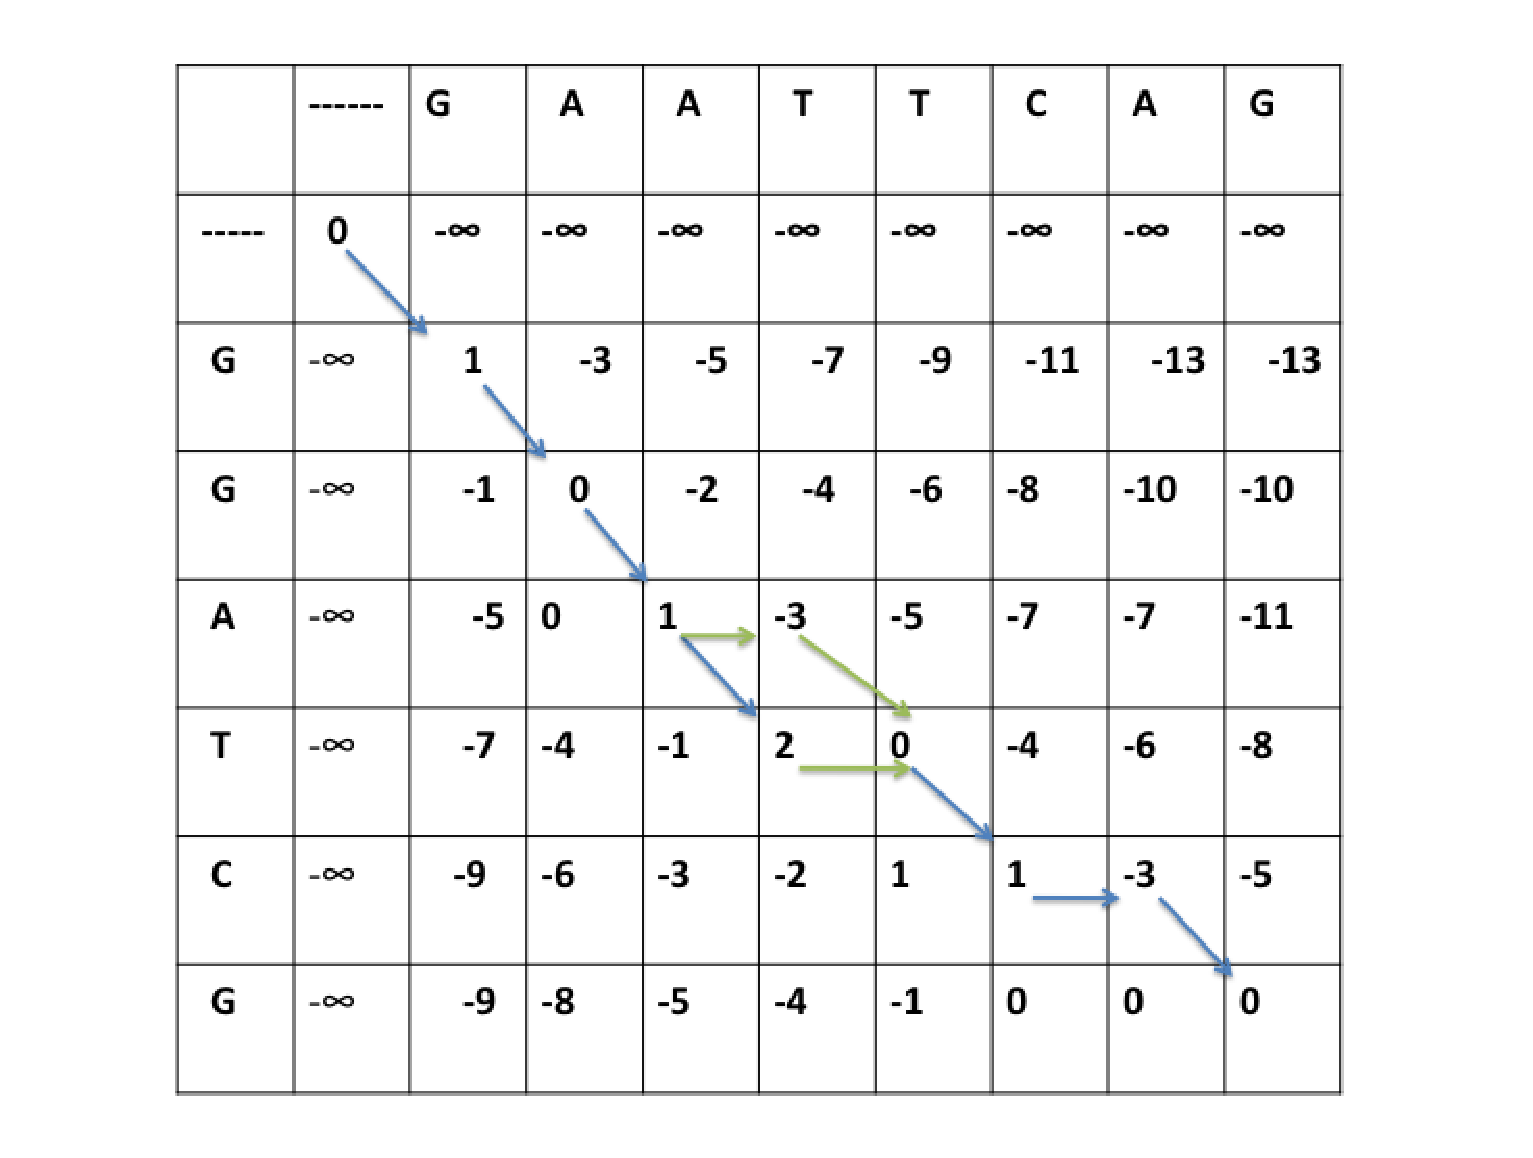
\includegraphics[width=4in]{Slide1}\caption{The matrix for the match state}
\par\end{centering}
\end{figure}

\begin{figure}
\begin{centering}
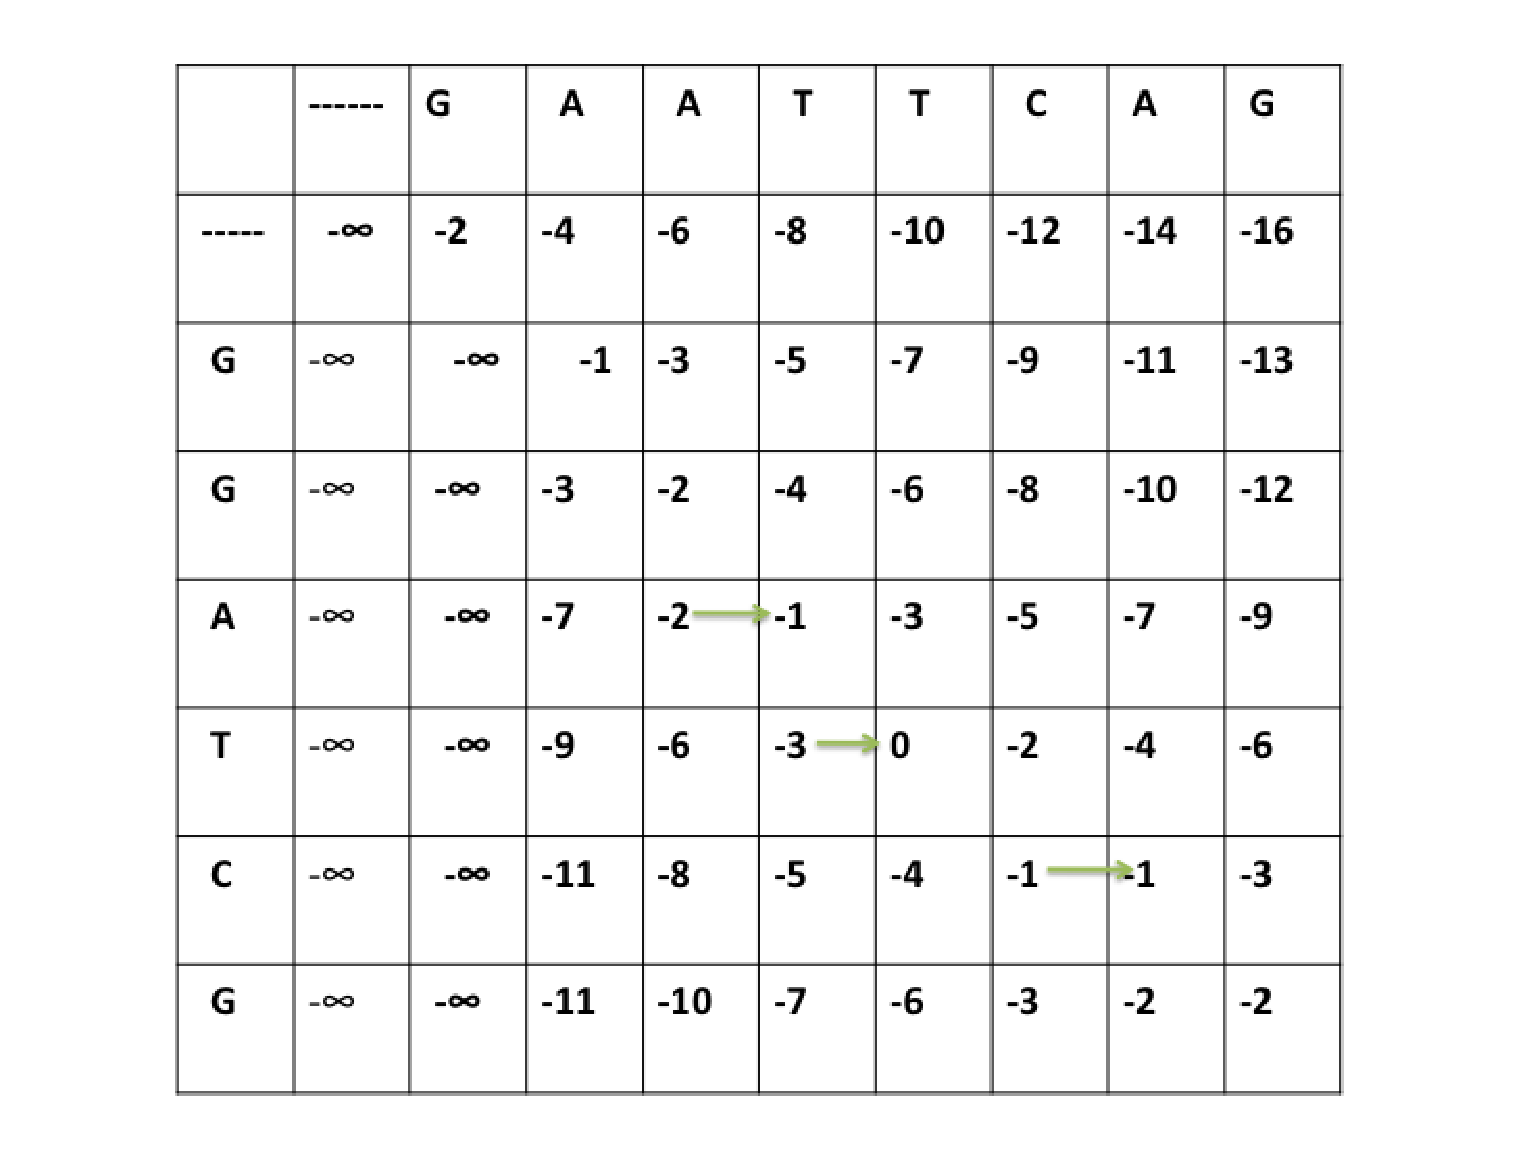
\includegraphics[width=4in]{Slide2}
\par\end{centering}
\caption{Matrix for deletion state}
\end{figure}

\begin{figure}
\begin{centering}
\caption{Matrix for insertion state}
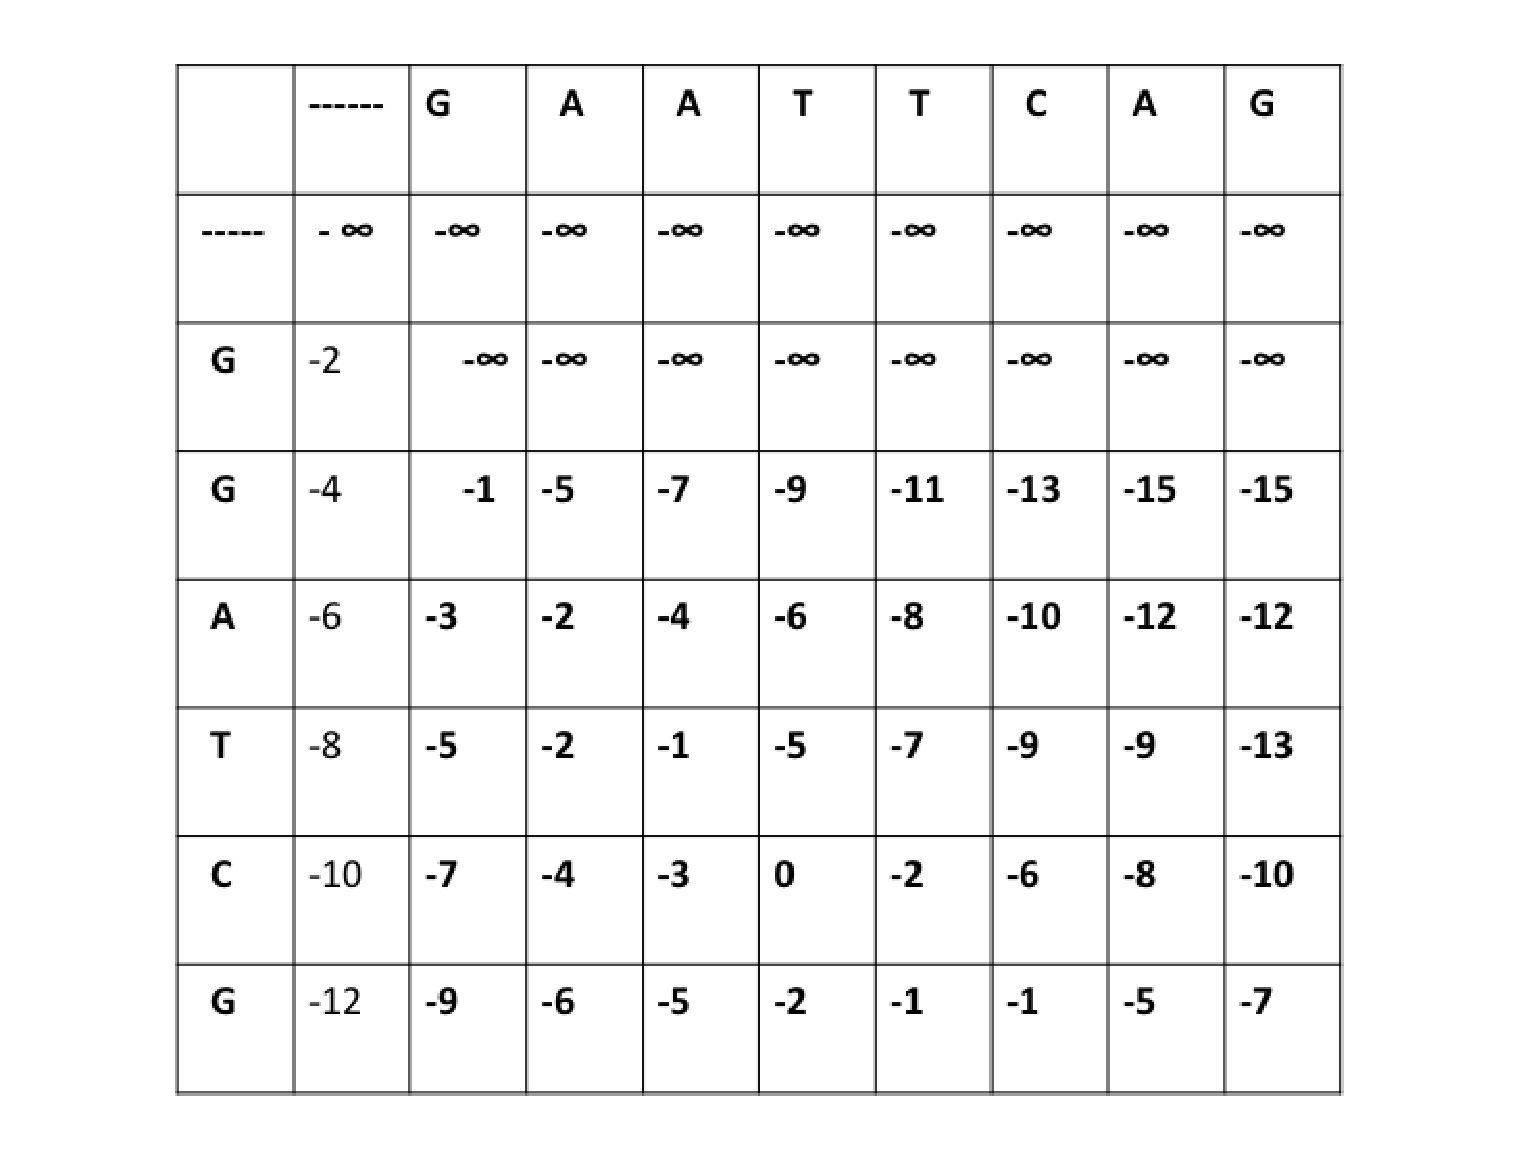
\includegraphics[width=4in]{Slide3}
\par\end{centering}
\end{figure}

\begin{figure}
\begin{centering}
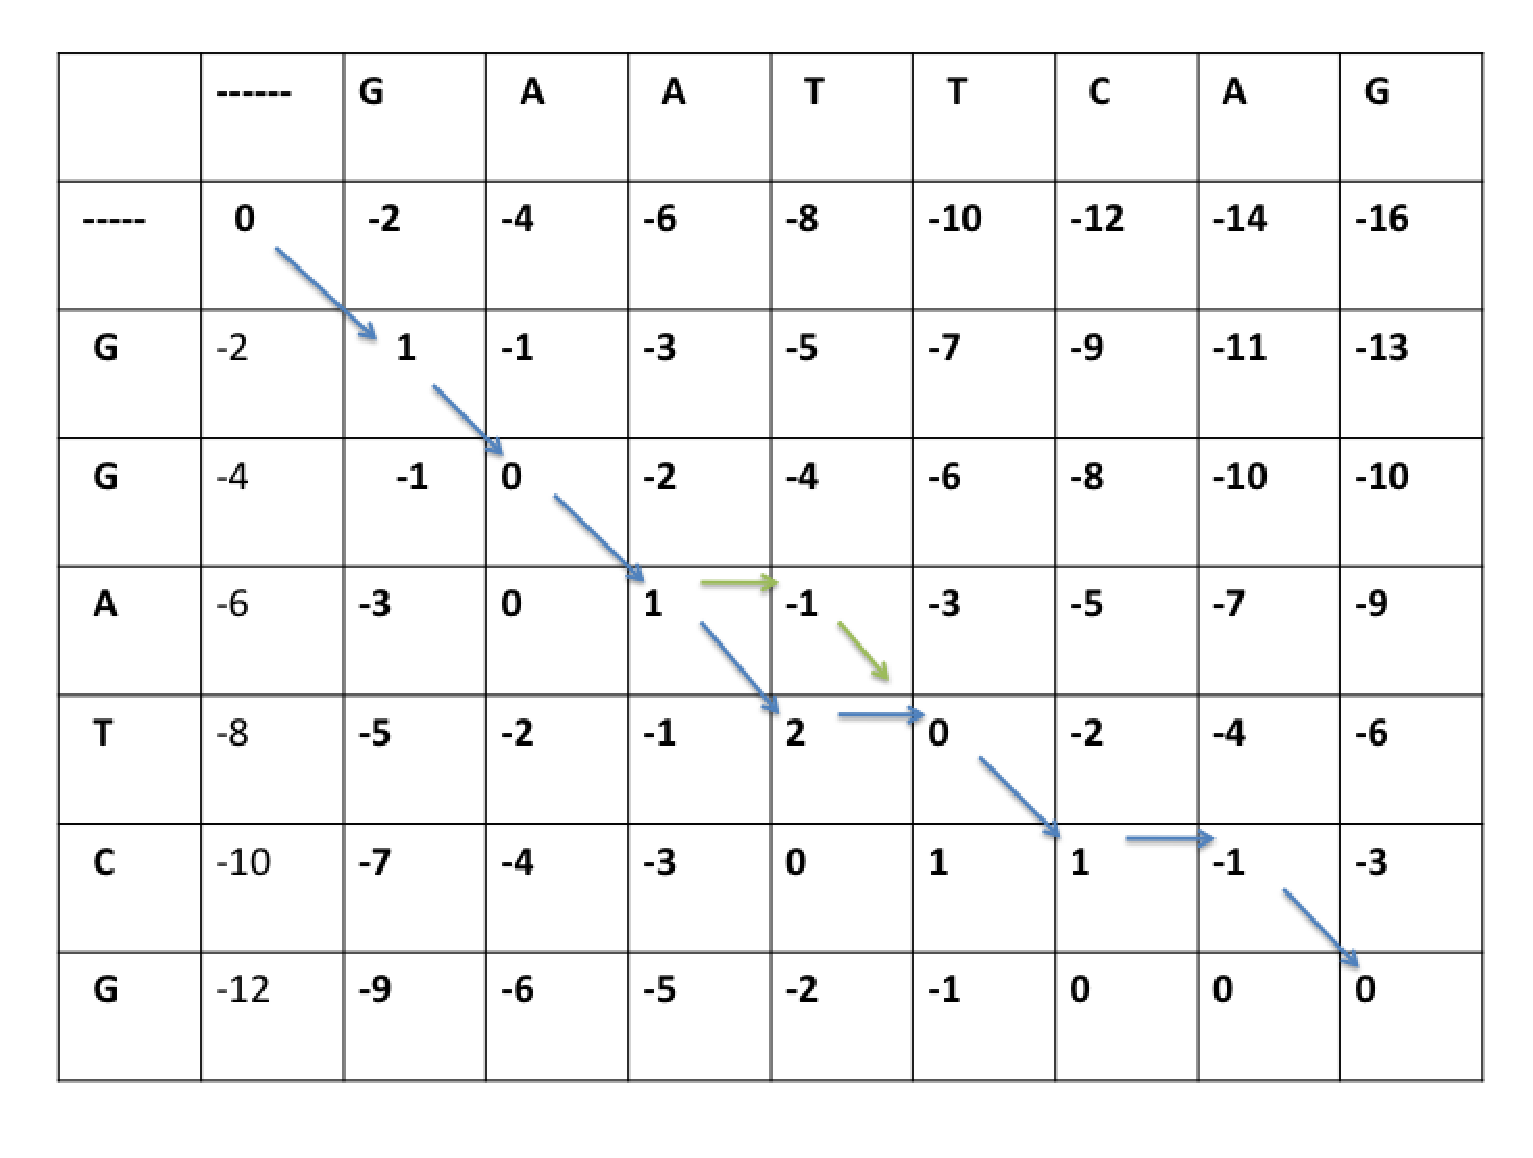
\includegraphics[width=4in]{Slide4}\caption{Alignment by backtracking}
\par\end{centering}
\end{figure}

There are two possible optimal alignments.

\begin{figure}
\begin{centering}
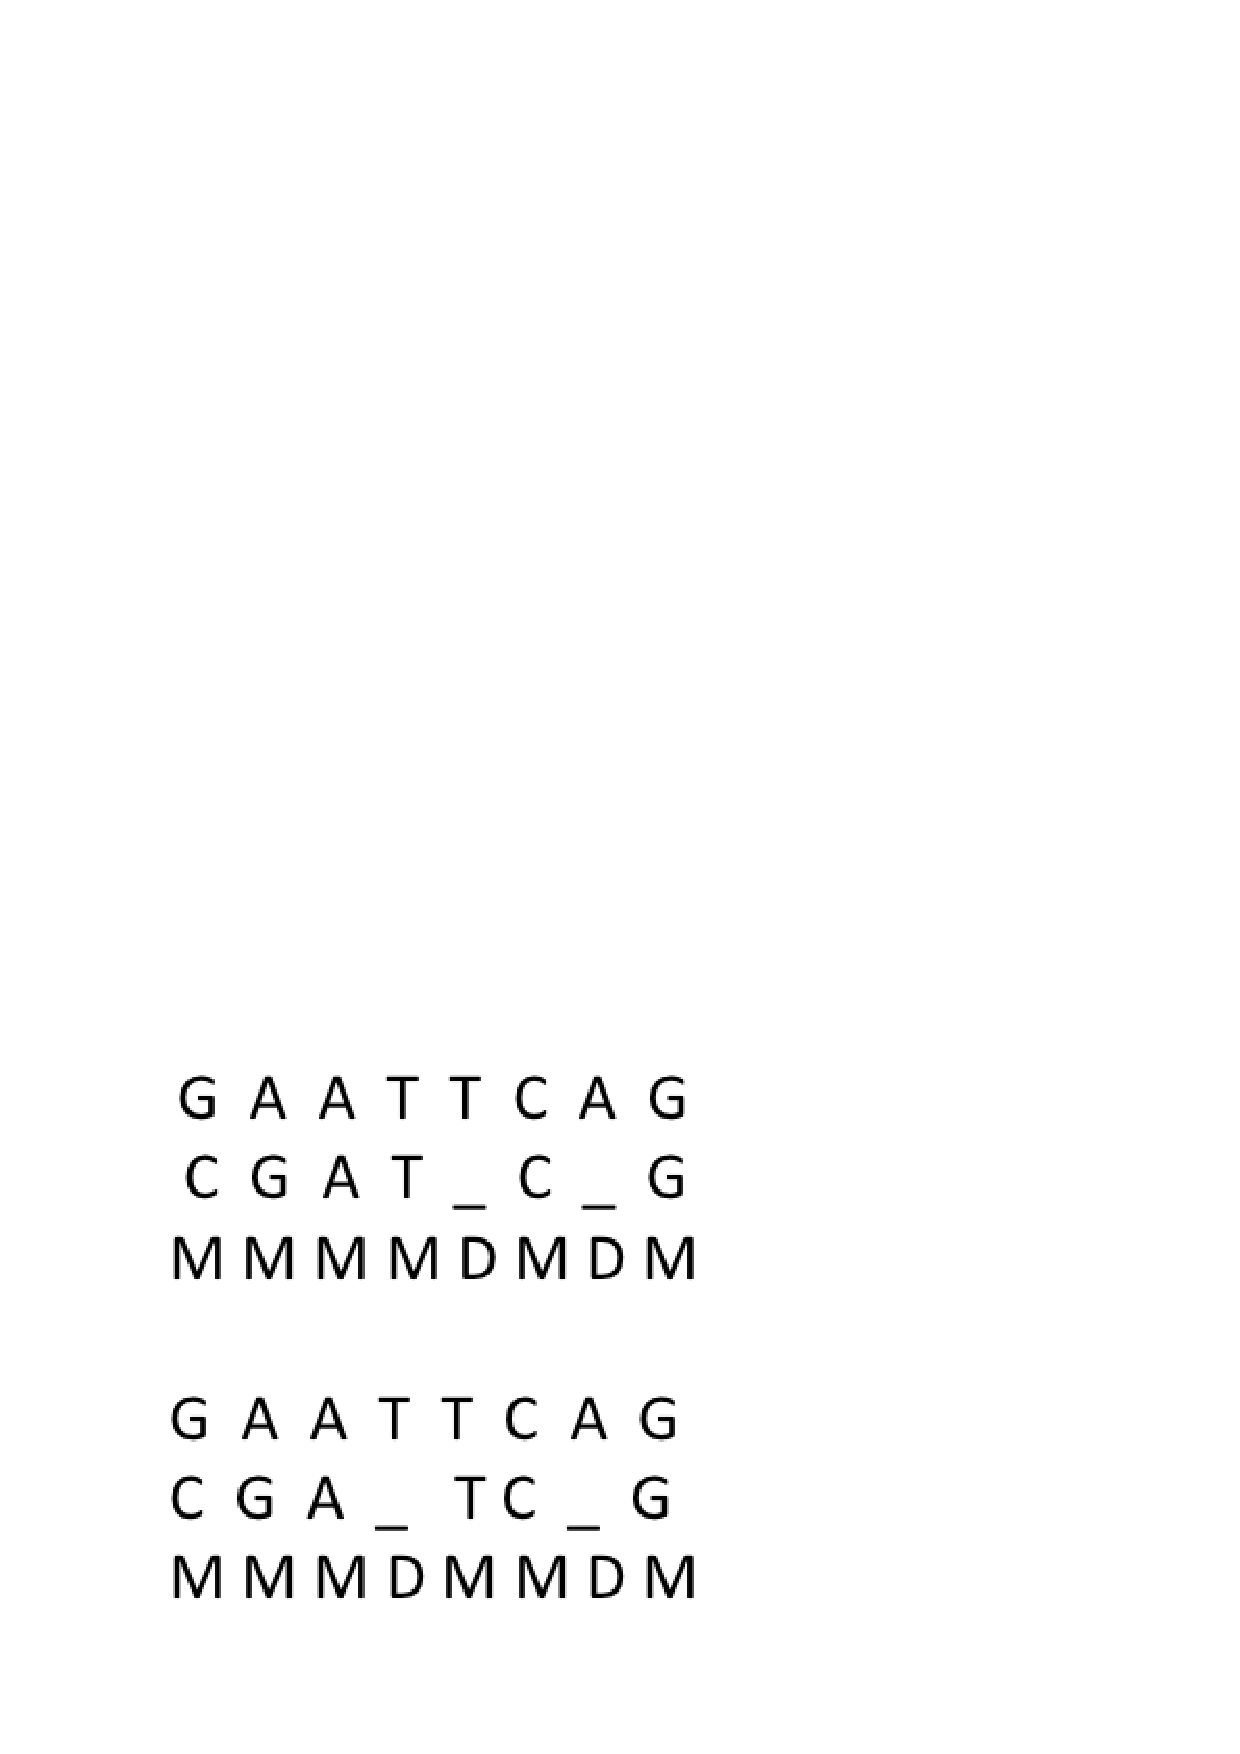
\includegraphics[width=2in]{alignment2.png}
\par\end{centering}
\caption{The alignments}
\end{figure}

\end{document}
>>>>>>> dad2d5cb564b29457f90cfb3187b371beb911d1d
